\chapter{Complete examples of \SBGNERLone maps}

The following maps present complete examples of SBGN \ERs representing biological processes. They by no mean exhaust the possibilities of  \SBGNERLone.

\fig{PCR} presents the different relations between the four entities involved in a Polymerase Chain Reaction (PCR). This examplifies the use of the \glyph{entity}, the logical operator \glyph{or}, the \glyph{state variable} ``existence'', the \glyph{unit of information}, as well as the relationships \glyph{interaction}, \glyph{assignment}, \glyph{necessary stimulation} and \glyph{absolute inhibition}.

\begin{figure}[htb]
\begin{center}
\scalebox{0.5}{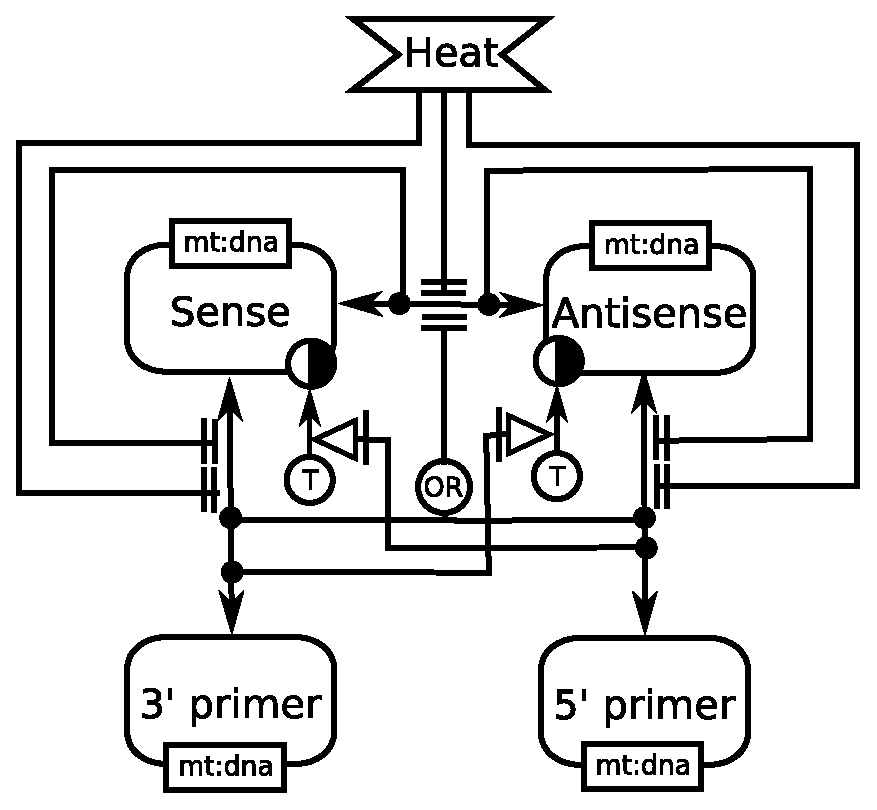
\includegraphics{examples/PCR}}
\caption{Principle of the Polymerase Chain Reaction.}\label{fig:PCR}
\end{center}
\end{figure}

